\documentclass[12pt]{article}
\usepackage{graphicx}
\usepackage{fullpage}
\usepackage{float}
\usepackage[symbol]{footmisc}
\graphicspath{{images/}}
\usepackage{natbib}
\bibpunct{(}{)}{;}{a}{,}{,}
\usepackage{titlesec}% http://ctan.org/pkg/titlesec
\title{An Attempt to Map the Magellanic Stream}
\author {
Kevin Yu
}

\begin{document}
\maketitle
\nocite{Heiles}
\begin{abstract}
We attempt to map the velocity of the Magellanic Stream with respect to the motion of the Earth by measuring the doppler shift of the 21 cm line. We observe the Magellanic Stream in a grid of 52 pointings, separated by $2^\circ$ each. Due to limited observing time, the noise level in our spectra are found to be on the order of the expected signal; however, our calibration techniques were not exact enough and likely contributed errors much larger than the noise itself. In the end, our velocity map for the Magellanic Stream cannot be trusted but with improved calibration techniques it should be possible to form a better velocity map.
\end{abstract}

\section{Introduction}
\subsection*{21cm Line}
The 21 cm emission line arises from a tranition between states in the hyperfine structure of neutral Hydrogen (HI). The 21 cm line corresponds to a an energy of $5.87$ $\mu$eV, the energy difference between the state of parallel electron and proton spin and the state of antiparallel spins. The characteristic time for this transision to occur is on the order of megayears, but the abundance of neutral Hydrogen in our universe makes this transition a common occurence and an excellent tracer of HI gas in our galaxy. We can map out the distribution of HI gas in and around our galaxy by making observations of the 21 cm line, as well as infer velocities relative to the motion of the Earth by the doppler shift of the line.

The rest frame wavelength of the transision is $1420.4$ MHz. For sources within and around our galaxy, observations of the line shifted from this center wavelength are indicative of motion of the HI along our line of sight.

\subsection*{The Magellanic Stream}
The Magellanic Stream consists of clouds of gas extending out from the Large Magellanic Cloud and the Small Magellanic Cloud, produced by the gravitational interactions between the Clouds and the Milky Way. It is located around the Galactic south pole. In this report, we use the 21 cm emission line to map out the overall motion of the HI gas in the Magellanic stream.

\section{Equipment}
To make our observations, we use a fragile radio telescope situated atop the scenic hills of Lafayette, CA, at Leuschner Observatory. This telescope consists of a 3.6m dish and dipole antennae calibrated for $\sim21$ cm radiation. The antenna itself is connected to a noise diode which can be turned on and off. When on, it injects $T=100\mathrm{K}$ noise which contributes to the spectrum uniformly at all temperatures. This is allegedly useful for calibration, as will be discussed in the next section.

The signal we receive is down-converted with a local oscillator and a $145\ \mathrm{MHz}-155\ \mathrm{MHz}$ bandpass filter. The signal is then digitized at a sample rate of 24 MHz. The sampled signal is transformed using a FIR filter in the IBOB to produce the signal in the frequency domain. This system takes one spectra roughtly every 0.7 seconds.

\section{Method}

\subsection*{Coordinates Selection}
The Magellanic Stream spans a large region of space around the Galactic south pole, as can be seen in Figure \ref{fig:mag-map}. In terms of Galactic longitude, $l$, and latitude, $b$, the Stream can be seen in the region from $b=-90^\circ$ to $b\approx-45^\circ$ and $l\approx-90^\circ$ to $l\approx90^\circ$. In order to optimize our observation time, we select a subsection of the above, focusing on areas which are known to feature HI gas more prominently. The Magellanic Stream is very faint with a expected signal on the order of $0.1\mathrm{K}$, so a long integration time is required.

\begin{figure}[H]
\center{
  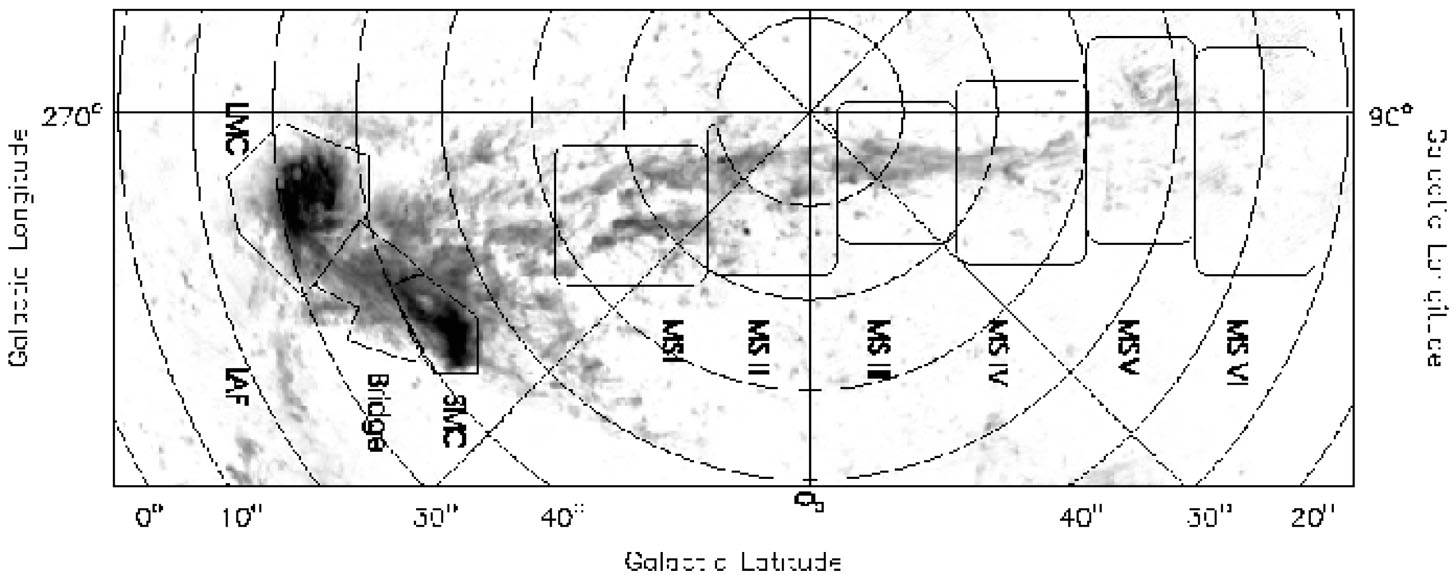
\includegraphics[width=400px]{ppnmagnhi}
}
\caption[SODUMB]{HI column density map of the Magellanic Clouds and the Magellanic Stream from \citet{Putman2003}. Most of the region on the left side of the map is not viewable from our vantage point in the northern hemisphere. The region we will sample is primarily contained in the box labelled MS III. According to Putman et. al., the velocity of the gas shown in this image relative to the Local Standard of Rest ranges from $\sim
+400\ \mathrm{km\ s^{-1}}$ at the LMC and SMC, to $\sim-400\ \mathrm{km\ s^{-1}}$ at the opposite edge of the stream.
}
\label{fig:mag-map}
\end{figure}

We would like to spatially sample twice per half-power beamwidth in order to capture structural information of the sky while avoiding redundant information; for our equipment this corresponds to $\sim4^\circ$. Due to the spherical geometry of the Galactic coordinate system, spacing our sampled points by $2^\circ$ requires a grid of points separated by $\Delta{b}=2^\circ$ (galactic latitude) and $\Delta{l}=\frac{2^\circ}{\cos{b}}$ (galactic longitude).

Our grid generated in this manner is show in Figure \ref{fig:grid}. In order to prevent large telescope adjustments between pointings, our observation script tends to select the next (available) pointing by following the line shown.

\begin{figure}[H]
\center{
  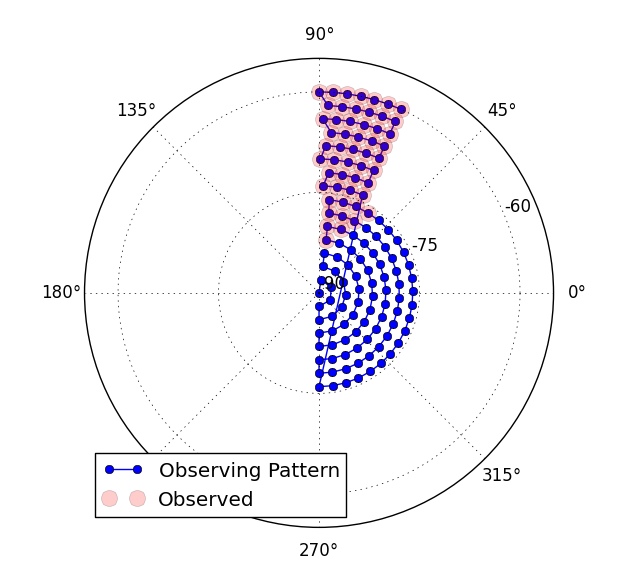
\includegraphics[width=300px]{zoop}
}
\caption[SODUMB]{Our grid generated with points separated by $2^\circ$. Points marked are pointings that were observed at least once by our script, which prioritizes low-declination sources when they are up. The line connecting the points shows the order in which points were prioritized (starting from the south galactic pole). Although the Magellanic Stream extends as far up as $-30^\circ$ in galactic latitude, we chose only to observe up to $-60^\circ$ due to limited time and the need for sufficient integration time per point.
}
\label{fig:grid}
\end{figure}

It is apparent from Figure \ref{fig:grid} that due to the low declination of these coordinates, many locations in the Galactic stream are simply not observable from our position in the northern hemisphere. Many other points of interest are only up for a limited amount of time per day. Figure \ref{fig:whatsup} shows the trajectory of the points across the Berkeley sky against the telescope pointing limits for April 29, 2014. Our observations were taken in a span of a week, from April 28, 2014, to May 4, 2014.

\begin{figure}[H]
\center{
  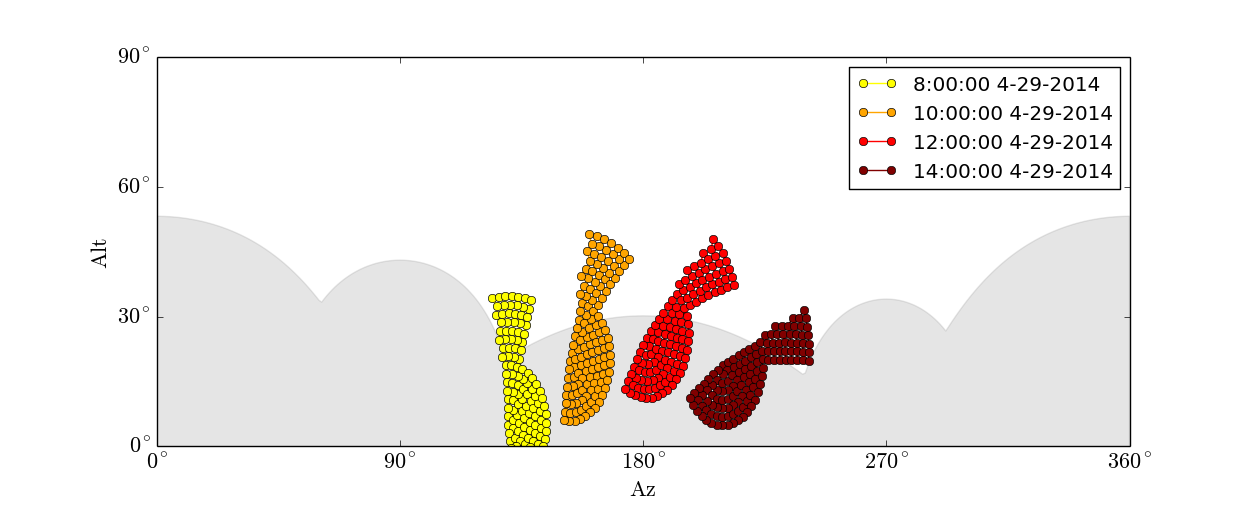
\includegraphics[width=440px]{trajectory}
}
\caption[SODUMB]{The trajectory of our grid across the sky on April 29, 2014, from our telesecope located at approximately $\mathrm{(37.92^\circ,\ -122.15^\circ)}$. The shaded region represents the pointing limits of the telescope; points in this region cannot be observed.
}
\label{fig:whatsup}
\end{figure}

\subsection*{LO Frequency}

Parts of the Magellanic Stream are moving relative to the LSR at -100 km/s to -400 km/s. These velocities will shift the observed frequency of the 21 cm line by an amount given by the doppler formula:
\begin{equation}
\nu = \nu_0 \left( 1 - \frac{v}{c} \right) \label{eq:doppler}
\end{equation}
For the velocities of the Magellanic Stream in the region we are observing, our signal \textit{should} fall in the range
\begin{equation}
1420.87\ \mathrm{MHz}< {\nu_{obs}} < 1422.29\ \mathrm{MHz} \label{eq:expected-freqs}
\end{equation}

Mixing an incoming signal at frequency $\nu$ with our local oscillator produces sidebands at $\nu \pm \nu_{LO}$. For the downconversion process described in Section 2, we want our signal to fall in the bandpass of the $145-155\ \mathrm{MHz}$ filter.

The Nyquist frequency of the ADC's 24 MHz sample rate is 12 MHz. Signals with frequencies greater than the Nyquist frequency are aliased, and appear in the spectrum reflected over that frequency. Thus, higher frequencies are mapped onto the $0-12\ \mathrm{MHz}$ range through a series of reflections. For example, signals in the range $12-24\ \mathrm{MHz}$ get mirrored over the Nyquist frequency and thus appear in reverse, while the range $24-36\ \mathrm{MHz}$ is mirrored twice and thus is mapped directly onto the $0-12\ \mathrm{MHz}$ range that we observe.

This pattern continues in this way, meaning that frequency ranges described by
\begin{equation}
(24n)\ \mathrm{to}\ (24n+12)\ \mathrm{MHz}\ [n = 1,2,...]
\end{equation}
are mapped without inversion onto our observed range. Specifically, the range $144-156\ \mathrm{MHz}$ (which includes the bandpass of our downconverter) is mapped unreflected into our observable spectrum.

For efficiency and calibration purposes (to be described in the next section), we want to select two LO frequencies; one that should see the frequencies in Equation \ref{eq:expected-freqs} only in the lower half of our frequency channels, and the other that only sees the signal in the upper half of our frequency channels.  An LO of frequency of $1273.6\ \mathrm{MHz}$ maps this range to the lower half of the bandpass ($147.27$ to $148.69\ \mathrm{MHz}$), while an LO frequency of $1269.6\ \mathrm{MHz}$ maps this range to the upper half of the bandpass ($151.27$ to $152.69\ \mathrm{MHz}$). This effect is depicted in Figure \ref{fig:lo}. Thus, the two LO frequencies we choose to use while observing are:
\begin{equation}
\nu_{LO} = 1269.6, 1273.6\ \mathrm{MHz} \label{eq:thelos}
\end{equation}

\begin{figure}[H]
\center{
  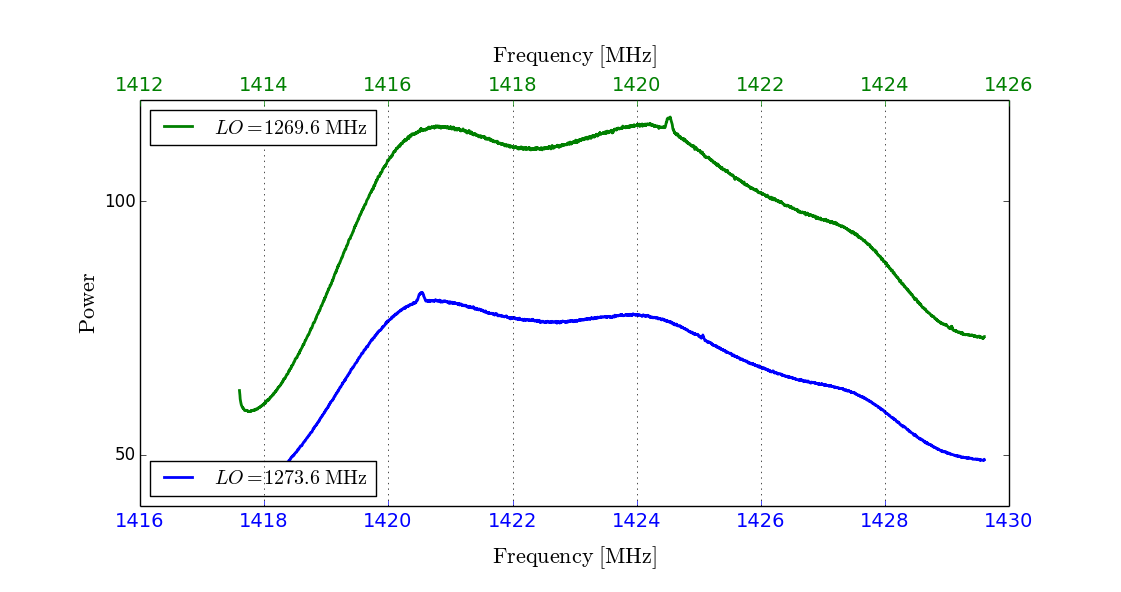
\includegraphics[width=450px]{lo_onoff_87_77-74}
}
\caption[SODUMB]{An example of captured spectra at our two LO frequencies. The converted frequency values for each LO setting are painstakingly labelled on the top and bottom of the plot. The prominent peak caused by HI emission within the Milky Way (at $\sim1420.5\ \mathrm{MHz}$) appears shifted in each spectra, but actually occurs at the same frequency value in both. The frequencies of interest are mapped onto the lower half of the bandpass for the higher LO, and mapped onto the higher half of the bandpass for the lower LO.
}
\label{fig:lo}
\end{figure}


\subsection*{Gain Calibration and Removing Bandpass}
The relevant calibration techniques for this project are described in detail by Carl Heiles in \textit{Calibrating the Intensity and Shape of Spectral Lines}. The idea is to take multiple spectra for each pointing at different settings in order to both identify and remove the bandpass shape as well as convert the spectra to physical units of temperature (Kelvin).

One spectrum is taken with the LO set such that the frequencies at which the signal is expected to appear are visible, which we call the ``on-line" spectrum. The power of this spectrum is described by this relationship:
\begin{equation}
P_{on}(\nu) = G(\nu) (T_{sys} + T_{HI}) \label{eq:pon}
\end{equation} 
In this equation, $P_{on}$ is the spetrum receieved, $G(\nu)$ is the gain of the system (assumed to be the same at all IF) that encapsulates the shape of the bandpass at different frequency channels, $T_{sys}$ is the temperature of the system, and $T_{HI}$ is the temperature of the HI signal.

The second spectrum is taken with the LO at the same setting (on-line), but with the $100\mathrm{K}$ noise diode turned on. This injects noise uniformly in frequency, so the power of this spectrum is described by:
\begin{equation}
P_{on, noise-on} = G(\nu) (T_{sys} + T_{HI} + T_{diode}) \label{eq:ponon}
\end{equation}

Finally, the method also requires a third spectrum with the noise diode turned off but the LO tuned to a frequency such that we capture a region of the spectrum that is ``off-line", or off of the expected HI emission line. This power spectrum is described by:
\begin{equation}
P_{off} = G(\nu) T_{sys} \label{eq:justtsys}
\end{equation}

By combining these three spectra, one can determine $T_{HI}(\nu)$, which is the quantity of interest. However, the method used by Heiles assumes that the system gain for both the on-line and off-line LO frequencies are the same, which is not actually the case. Thus, if we relax the assumption that the gain is independent, we need to modify the method to scale $P_{on}$ and $P_{off}$ to the same level, which includes taking the analogous measurement to Equation \ref{eq:justtsys} for the on-line LO frequency.

The result of this, following similar steps to those laid out in the source, gives us a theoretical expression for $T_{HI}(\nu)$:
\begin{equation}
T_{HI}(\nu) = \left(\frac{P_{on}(\nu)}{P_{off}(\nu)} \frac{G_{off}}{G_{on}} - 1\right)T_{sys} \label{eq:T-hi}
\end{equation}
$G_{off}/G_{on}$ is the ratio of the gains at the two LO frequencies. To get this quantity, we take the difference between Equations \ref{eq:ponon} and \ref{eq:pon} for both the on and off LO frequencies.
\begin{equation}
\frac{G_{off}}{G_{on}} \approx \frac{\Sigma{(P_{off,noise}(\nu) - P_{off}(\nu))}}{\Sigma{(P_{on,noise}(\nu)- P_{on}(\nu))}} \label{eq:gains}
\end{equation}
The system temperature can be found using the Heiles paper, replacing $P_{off}$ with $P_{on}$ and making sure to exclude the ranges that we expect HI to appear; i.e. exclude the frequencies of Equation \ref{eq:expected-freqs} as well as the frequencies near line-center, $1420.4\ \mathrm{MHz}$.
\begin{equation}
T_{sys} \approx \frac{\Sigma{P_{on}(\nu)}}{\Sigma{(P_{on,noise}(\nu)-P_{on}(\nu))}}\ \mathrm{(excluding\ HI\ ranges)} \label{eq:tsys}
\end{equation}
Putting Equations \ref{eq:gains} and \ref{eq:tsys} into Equation \ref{eq:T-hi} shows us how to combine our spectra to get the temperature of the HI signal.

By using the two LO frequencies in Equation \ref{eq:thelos}, we can divide the spectra we collect into two halves; the half including the signal as the ``on-line" spectrum and the half excluding the signal as the ``off-line" spectrum. Thus, we double our efficiency by using every observation as a ``off-line" and an ``on-line" spectrum simultaneously. 

\subsection*{Removing Interference}
The raw spectra features many large amplitude spikes with width of usually no more than a few frequency channels, often the spikes only have the width of a single channel. To remove these features, we apply to every spectra a median boxcar filter of width N=10. This is a narrow filter corresponding to a width of $0.015\ \mathrm{MHz}$, which is much smaller than the expected width of any spectral features we expect to see, but wide enough to flatten out the RFI that happens to span a few adjacent frequency channels.

\subsection*{Observing}
Our goal is to generate a mapping from $(l, b)$ coordinate pairs to the spectal data generated by observing those points. For a particular pointing, we reduce noise by averaging arrays of spectral data generated over a certain period of time. We integrate for a total of four minutes per pointing at a time. For our script and equipment settings, this corresponds to averaging $N=358$ spectra per pointing. Because the Magellanic Stream is faint, four minutes per pointing is not quite enough time to see the 21 cm line from the source. However, with enough telescope time, we will measure spectra for pointings multiple times and increase the number of samples averaged, $N$. This will reduce the noise by a factor of $\sqrt{N}$, and we should be able to make out the spectral features with enough observation time.

The pattern our observation sessions are are as follows:
\begin{enumerate}
\item Select a new point and point the dish to that position in the sky.
\item Take spectra for about two minutes (179 spectra) with the noise diode off and LO frequency set to $\nu_{LO} = 1273.6$ MHz. 
\item Take spectra for twenty seconds (29 spectra) with the noise diode on and the LO frequency set to $\nu_{LO} = 1273.6$ MHz.
\item Update the azimuthal coordinates of the point and repoint the dish to that position.
\item Take spectra for two minutes (179 spectra) with the noise diode off and LO frequency set to $\nu_{LO} = 1269.6$ MHz. 
\item Take spectra for twenty seconds (29 spectra) with the noise diode on and the LO frequency set to $\nu_{LO} = 1269.6$ MHz.
\end{enumerate}

\subsection*{Peak Detection to Average Velocity}
In order to extract an average velocity from the calibrated spectra generated from Equation \ref{eq:T-hi}, we take the mean of the doppler velocity of each frequency channel, weighted by the power received in that channel. We apply this to only the range of frequencies described in Equation \ref{eq:expected-freqs}, excluding contributions from our own Milky Way\footnote{Contributions from our own Galaxy should be near line-center because, looking at the galactic south pole, we are looking through gas that is moving at a similar velocity to us on Earth.}. Results of this can be seen in the next section in Figure \ref{fig:velocities}.

\section{Results}

\subsection*{A Calibration Disaster}
We calibrate spectra by applying the methods in Section 3 and Equation \ref{eq:T-hi} to slices of the spectra in the region of interest. However, this results in the extremely not-flat baslines seen in left-hand column of Figure \ref{fig:calibration}. Although theoretically the shape of the bandpass should have been removed using the calibration techniques described earlier, there must be some variation in the parameters as a function of time or IF frequency. Thus,  application of Equation \ref{eq:T-hi} does not fully remove the shape of the baseline. The very visible peak at $1420.5\ \mathrm{MHz}$ is unfortunately not the signal we are trying to locate; the signal we are looking for exists somwhere in the region just to the right of it.

In order to remove the baseline shape from this stage, we fit a third degree polynomial to the regions of the spectra below the prominent HI peak ($\nu < 1420.2\ \mathrm{MHz}$) and above the range of frequencies we expect to see from the Magellanic Stream ($\nu > 1422.6\ \mathrm{MHz}$). The purpose of this is to approximate the shape of the baseline and subtract it from our signal. However, due to the severely fluctuating shape of the baseline (a particularly bad example can be seen in the fifth row of Figure \ref{fig:calibration}), there is no good reason in most cases to trust that this third degree polynomial is a true reflection of the shape. Using a higher degree polynomial would likely overfit the data, and fitting to a larger data range runs the risk of fitting the polynomial to the actual spectral features; this would wipe out the signal we are trying to observe.

\begin{figure}[H]
\center{
  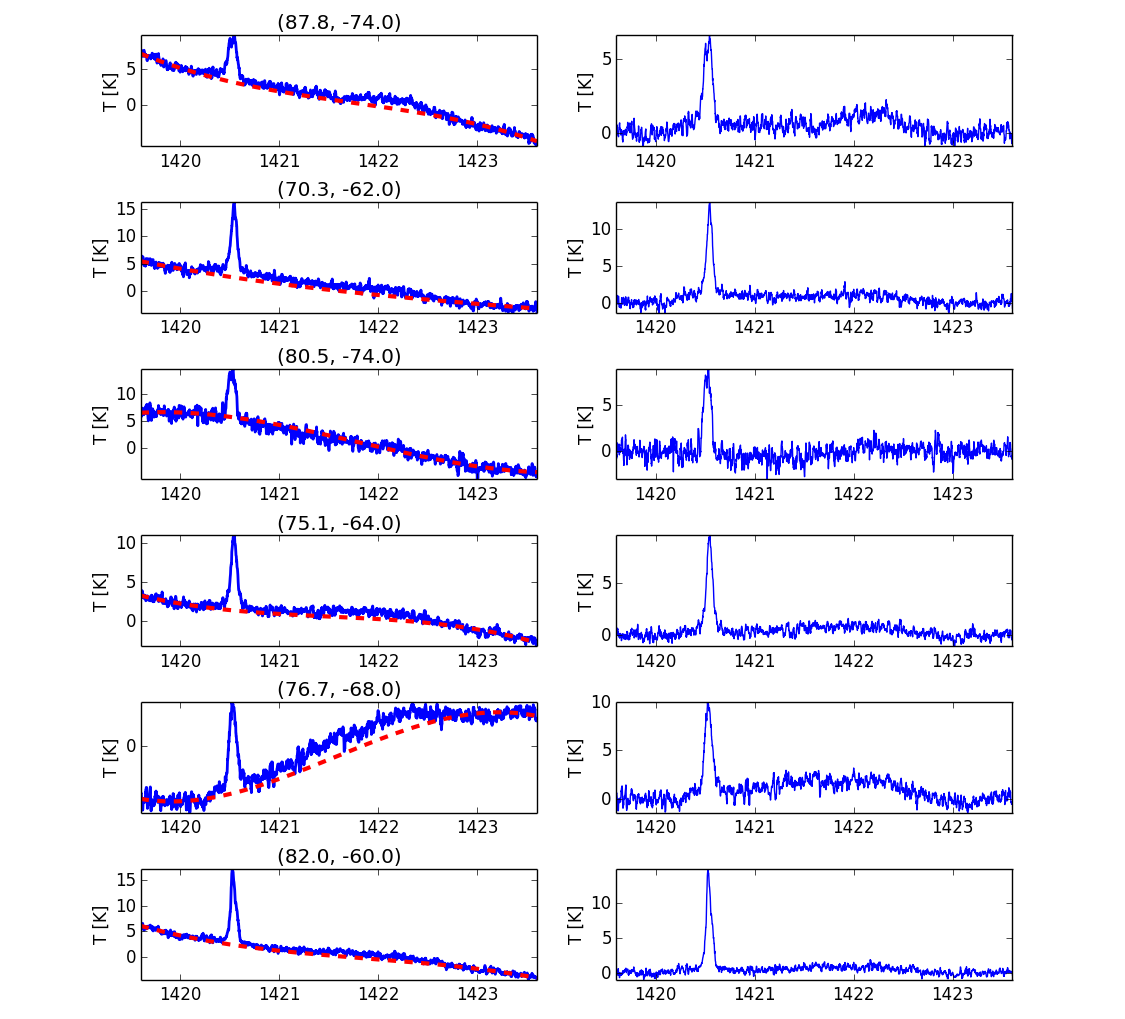
\includegraphics[width=400px]{calibration}
}
\caption[SODUMB]{An sampling of the calibration results for our spectra. Left: Spectra calibrated using Equation \ref{eq:T-hi}, with a third degree polynomial fitted to the data at the ends (outside of the expected HI contribution). Though some look passable, it is clear from spectra that the shape is too strange to be fit cleanly by our polynomial. Right: The same spectra with the polynomial fit subtracted off. Though some appear to feature an increase in power at the frequencies of interest, the shallow hump is likely just an artifact of this poor fit.
}
\label{fig:calibration}
\end{figure}

\subsection*{Integration Time and Noise Estimates}
Due to the trouble calibrating, it seems useful at this point to analyze the contributions of noise to our data and see whether our data is at a stage at which we should be able to make out an emission line from the Magellanic Stream. According to the lab manual, the line should be on the order of a few tenths Kelvin.

The amount of time we integrated for at each point is shown as a heat map in Figure \ref{fig:noises}. The lab manual suggests that a minimum of 10 minutes (600 seconds) per point is necessary to make out a signal from the Magellanic Stream. Most points we observed fall short of this threshold, although a couple of points were averaged for about 800 seconds.

On the right of Figure \ref{fig:noises} is a heatmap of the noise level (in Kelvin) for spectra taken at each of these points. We estimate the noise level at a particular pointing by taking the section of the calibrated and averaged spectra (as in the right column of Figure \ref{fig:calibration}) corresponding to the frequency channels of interest of Equation \ref{eq:expected-freqs}. We flatten this section by subtracting from it a median filtered version of itself, then determine the characterstic scale of the noise by taking the standard deviation of this result. The noise level is for the most part between $0.1$ and $0.4\ \mathrm{K}$, which is on the order of the expected signal from the Magellanic Stream. Thus, at these noise levels we expect a signal-to-noise ratio of $\sim1$. In contrast, the signal-to-noise ratio for the Milky Way's HI peak in most of our spectra is $\sim100$, and is easily visible in Figure \ref{fig:noises}. 

\begin{figure}[H]
\center{
  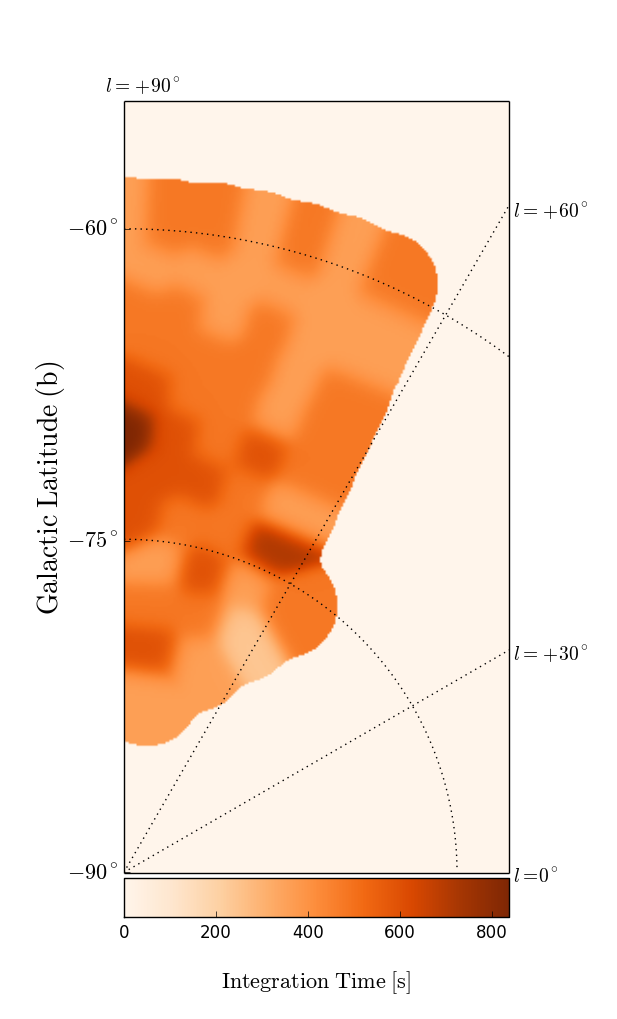
\includegraphics[width=200px]{integrationtime}
    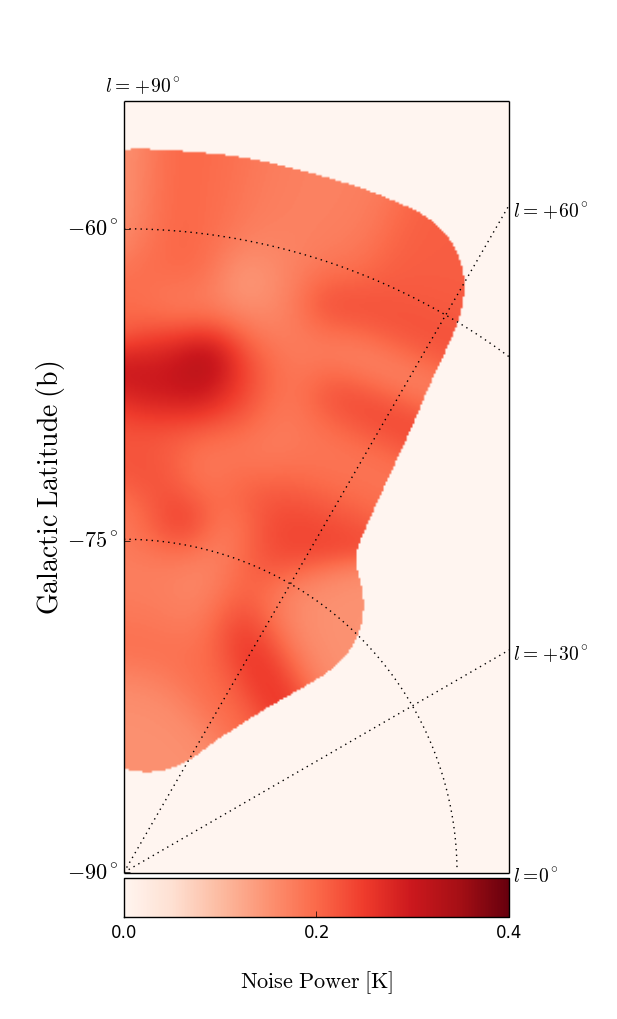
\includegraphics[width=200px]{noise}
}
\caption[SODUMB]{Left: Heat map of amount of integration time per point. Right: Noise level of the calibrated spectra at each point. The noise is on the order of the expected signal ($\sim 0.1\mathrm{K}$); however, one might imagine that the Magellanic Stream signal should still be visible given proper calibration techniques. However, our polynomial fit to the spectral baseline probably includes systematic errors greater than our noise level; Thus, our problem with generating clean spectra is likely more due fitting to the bandpass shape than the noise level itself.
}
\label{fig:noises}
\end{figure}

Compared to the level of our noise, the error introduced by our polynomial fits is more more significant. Although we can improve our signal by increasing our integration/observation time, our calibration technique would still have to be improved greatly in order to make out Magellanic Stream data.

\subsection*{Velocity Map}
Despite the issues raised above, we move onward in our quest to make a map of the velocity of the Magellanic Stream, while keeping in mind that the data here is not very trustworthy. By applying the method described in Section 3 of taking a weighted average of the velocities at each frequency channel over the range in Equation \ref{eq:expected-freqs}, we produce velocities at each pointing, and map them out in Figure \ref{fig:velocities}.

\begin{figure}[H]
\center{
  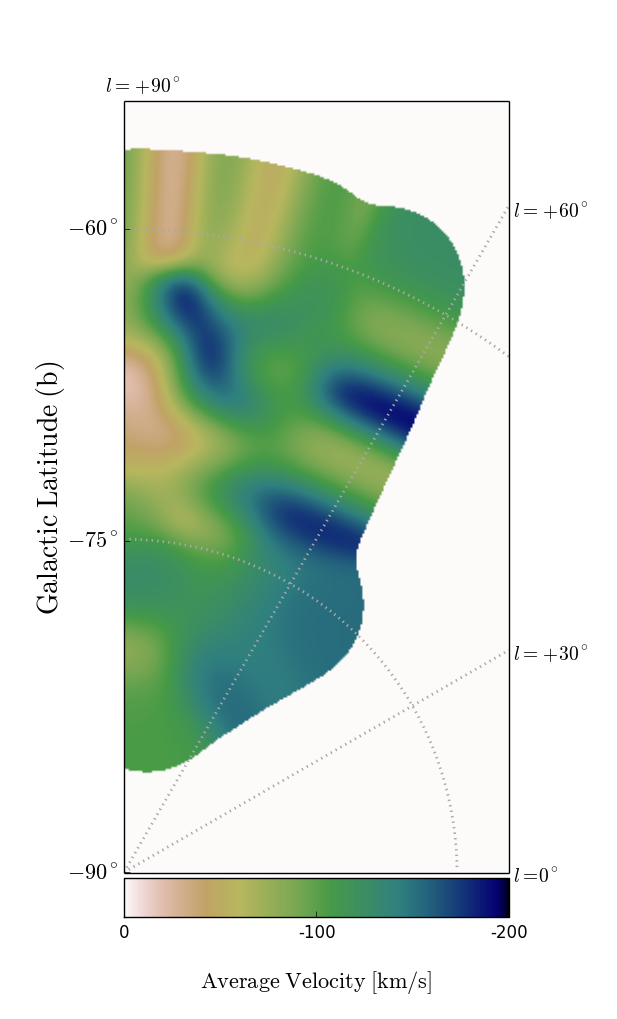
\includegraphics[width=200px]{velocities}
}
\caption[SODUMB]{Map of the velocity of the Magellanic Stream relative to Earth. Due to the issues raised about the calibration and noise, the velocity map cannot be trusted to be accurate; but if it were, the velocities in this field reach about $-200\ \mathrm{km\ s^{-1}}$.
}
\label{fig:velocities}
\end{figure}

\section{Conclusion}
We find that calibration techniques are extremely vital in extracting weak signals. The straightforward methods of calibration outlined by Carl Heiles did not apply directly to our case, and our adapted calibration method did not result in perfect alignment between ``on-line" and ``off-line" spectra. Thus, we were required to fit a polynomial to the baseline which introduced a great amount of uncertainty in our final dataset. Improving on the calibration would be a vital step in improving the quality of our map, moreso than decreasing the noise level---which we found to generally be small enough to give us a signal-to-noise ratio of $\sim1$.

One possible explaination for the discrepancy between the on-line and off-line spectra could be system parameters changing during the somewhat long integration time of four minutes (two minutes ``on-line", and two minutes ``off-line"). It is possible that factors like the system temperature change enough during that time to throw off the Equations \ref{eq:pon}, \ref{eq:ponon}, and \ref{eq:justtsys}. It is possible that shorter pointing time would help improve calibration by reducing the time between taking the two spectra used to calibrate each other. However, this would come at the cost of spending slightly more time repointing the telescope.

Finally, we learn the important lesson of starting early on projects for which it is known beforehand that many pointings and long integration times are needed.

\section{Acknowledgement}
I would like to use this space to acknowledge the fact that I am very sleepy now, and it is time for me to go to sleep.

MVP of this lab goes to Karto (Figure \ref{fig:kartp}) for driving up and down to the telescope to fix it repeatedly. Second MVP is the half-day extension, which was extremely clutch. Plotting was done using matplotlib and numpy modules, and 2-D convolutions were done with the help of the astropy module for Python.


\bibliographystyle{plainnat}
\bibliography{myBib.bib}

\newpage
\begin{figure}[H]
\center{
  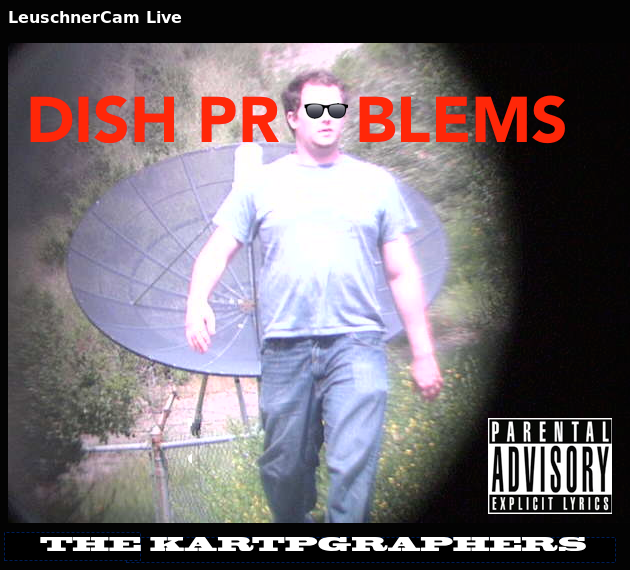
\includegraphics[width=450px]{dishproblems}
}
\caption[SODUMB]{Dish Problems - The Kartpgraphers.}
\label{fig:kartp}
\end{figure}


\end{document}